\documentclass[12pt,oneside]{book}
\usepackage{xcolor}
\usepackage{tikz}
\usetikzlibrary{calc}
\usepackage{multicol}
\usepackage{titletoc}
\usepackage{ragged2e}
\usepackage{fancyhdr}
\usepackage{url}
\usepackage{verbatim}
\usepackage[utf8]{inputenc}
\usepackage{float}
\usepackage{titlesec}
\usepackage{lmodern} % for bold teletype font
\usepackage{setspace}
\usepackage{blindtext}
\usepackage{mathptmx}
\usepackage{listings}
\usepackage{caption}

\DeclareCaptionFont{white}{\color{white}}
\DeclareCaptionFormat{listing}{%
	\parbox{\textwidth}{\colorbox{gray}{\parbox{\textwidth}{#1#2#3}}\vskip-4pt}}
\captionsetup[lstlisting]{format=listing,labelfont=white,textfont=white}
\lstset{frame=lrb,xleftmargin=\fboxsep,xrightmargin=-\fboxsep,
	basicstyle=\ttfamily,
	columns=fullflexible,
	breaklines=true,}

\titleformat*{\section}{\large\bfseries}
\titleformat{\chapter}[display]
  {\normalfont\Large\bfseries}{\filright\chaptertitlename\ \thechapter}
  {20pt}{\Large\filcenter}
\titlespacing*{\chapter}{0pt}{-30pt}{40pt}

\usepackage[bookmarks, colorlinks=false, pdfborder={0 0 0}, pdftitle={<pdf title here>}, pdfauthor={<author's name here>}, pdfsubject={<subject here>}, pdfkeywords={<keywords here>}]{hyperref}

\usepackage{etoolbox} % enable fancyhdr on chapter pages.
\patchcmd{\chapter}{\thispagestyle{plain}}{\thispagestyle{fancy}}{}{}
\patchcmd{\lstlisting}{\thispagestyle{plain}}{\thispagestyle{fancy}}{}{}

\renewcommand\bibname{References}

\pagestyle{fancy}
\fancyhf{}
\fancyhead[L]{COLLEGE DATABASE MANAGEMENT SYSTEM}
\fancyfoot[L]{RNSIT, Dept. of CSE}
\fancyfoot[R]{Page \thepage}

\renewcommand{\headrulewidth}{5pt}
\renewcommand{\footrulewidth}{5pt}
\newlength\FHoffset
\fancyheadoffset{\FHoffset}

\definecolor{darkbrown}{RGB}{153, 51, 51}
\definecolor{blue}{RGB}{102, 102, 255}
\definecolor{black}{RGB}{0, 0, 0}

\renewcommand{\headrule}{\hbox to\headwidth{\color{darkbrown}\leaders\hrule height \headrulewidth\hfill}}
\renewcommand{\footrule}{\hbox to\headwidth{\color{darkbrown}\leaders\hrule height \footrulewidth\hfill}}


\renewcommand{\contentsname}{\centering Contents}

\AtBeginDocument{%
  \addtocontents{toc}{\protect\thispagestyle{empty}}%
  \addtocontents{lof}{\protect\thispagestyle{empty}}%
}

\usepackage{geometry}
\geometry{
	lmargin = 1.25in,
	rmargin = 1in,
	top = 0.75in,
	bottom = 0.75in,
}
\definecolor{bg}{rgb}{0.95,0.95,0.95}


\begin{document}


\begin{titlepage}
\begin{center}

\begin{tikzpicture}[remember picture, overlay]
\draw[line width = 2pt] ($(current page.north west) + (1in,-1in)$) rectangle ($(current page.south east) + (-1in,1in)$);
\end{tikzpicture}
\break\break
\textup{\large {\textcolor{brown}{\bf VISVESVARAYA TECHNOLOGICAL UNIVERSITY} \\ {\textcolor{brown}{\bf BELGAVI-590014}}}}\\[0.1in]

\includegraphics[width=0.18\textwidth]{./VTU.png}\\[0.1in]
\textup{\small {\textcolor{black}{\textbf {A DMBS Mini-Project Report} \\ {\textbf {On}}}}} \\[0.2in]
\textup{\large {\textcolor{blue}{\textbf {\textit {``College Database Management System"}}}}} \\[0.2in]
\textup{{\textit {Submitted in partial fulfillment of the requirements for the 5th semester of} \\ {\textbf {\textit {Bachelor of Engineering in Computer Science and Engineering}} \\ \textit {of Visvesvaraya Technological University, Belgavi}}}}\\[0.15in]
\textup{Submitted by:}
\break\break
\begin{tabular}{l  l}
\textcolor{blue}{\textbf{Shivam Nagpal}} & \textcolor{blue}{\hspace{2.7cm}\textbf{1RN16CS098}}\\[0.3in]

\end{tabular}
\break\break\break\break
\textup{\normalsize {\textcolor{black}{ Under the guidance of:}}}\break\break
\begin{tabular}{l l l}
\textbf{Mr. K Sunil Kumar} & \hspace{0.7cm}\textbf{Mrs. A N Ramyashree} & \hspace{0.7cm}\textbf{Dr. H R Sashidhara}\\
\textbf{Assitant Professor} & \hspace{0.7cm}\textbf{Assitant Professor}  & \hspace{0.7cm}\textbf{Assitant Professor}\\
\textbf{Dept. of CSE} & \hspace{0.7cm}\textbf{Dept. of CSE}  & \hspace{0.7cm}\textbf{Dept. of CSE}\\[0.2in]
\end{tabular}


\includegraphics[width=3cm, height=3cm]{./RNS_logo.png}\\[0.1in]

\textup{\normalsize {\textcolor{brown}{\bf Department of Computer Science and Engineering} \\ {\textcolor{brown}{\bf \bf{RNS Institute of Technology}}}}}\\
\textup{\small {\textcolor{brown}{\bf Channasandra, Dr. Vishnuvardhan Road, Bengaluru-560 098}\\ \textbf {\textcolor{brown}{2017-2018}}}}
\end{center}
\end{titlepage}

\thispagestyle{empty}
\begin{center}

\begin{tikzpicture}[remember picture, overlay]
\draw[line width = 2pt] ($(current page.north west) + (1in,-1in)$) rectangle ($(current page.south east) + (-1in,1in)$);
\end{tikzpicture}
\break\break
\textup{\large {\textcolor{darkbrown}{\bf RNS Institute of Technology}} \\
{\normalsize{\textcolor{brown}{Channasandra, Dr. Vishnuvaradana Road,\\ Bengaluru-560 098}}}}\\[0.1in]
\textup{\normalsize {\textcolor{blue}{\bf DEPARTMENT OF COMPUTER SCIENCE AND ENGINEERING}}}\\[0.1in]

\includegraphics[width=3cm, height=3cm]{./RNS_logo.png}\\[0.1in]
\textup{\large {\textcolor{black}{\textbf {CERTIFICATE}}}} \\[0.1in]
\end{center}

\justify
\begin{tabular}{p{15cm}}
\hspace{0.4cm} Certified that the DBMS mini-project work entitled \textbf{``College Database Management System"} has been successfully carried out by \textbf{Shivam Nagpal} bearing USN \textbf{1RN16CS098}, bonafide student of \textbf{RNS Institute of Technology } in partial fulfillment of the requirements for the \textbf{5th semester Bachelor of Engineering} in \textbf{Computer Science and Engineering} of \textbf{Visvesvaraya Technological University}, Belagavi, during the academic year 2018-2019. It is certified that all corrections/suggestions indicated for Internal Assessment have been incorporated. The project report has been approved as it satisfies the mini-project requirements of DBMS lab of 5th semester BE in CSE.\\[0.7in]
\end{tabular}

\justify
\begin{tabular}{l l}
\textbf{Mr. Karanam Sunil Kumar} & \hspace{1.7in}\textbf{Dr. G T Raju}\\
\textbf{Assistant Professor} & \hspace{1.7in}\textbf{Vice Principal \& Head}\\
\textbf{Dept. of CSE} & \hspace{1.7in}\textbf{Dept. of CSE}\\[0.2in]
\end{tabular}
\\[0.3in]

\justify
\textup{\underline{\textbf{External Viva:}}} \\
\textup{\textbf{Name of the Examiners}}\hspace{6cm} {\textbf{Signature with date}} \\
\justify
\textup{\textbf{1.}} \\[0.4in]
\textup{\textbf{2.}}
\newpage

\pagestyle{empty}
\begin{center}
\textup{\large{\textbf{ABSTRACT}}}
\end{center}
\setstretch{1.5}
\justify
\indent
The 'College Database Management System' project has been developed with the view of maintaining records of all the Students, Professors, Departments and Subjects. The purpose of this project is to provide a user friendly system to store the data fast and securely with easy accessing and manipulation of the same.\\

The aim of this project is to manage details of the entities involved in a college. This project provides simple interaction to do basic operations on the details. It also provides very efficient searching throughout the database.\\

This project uses the MySql with InnoDB Engine as Database to store the details and JavaFX in the front-end for user interface. Java is used in the back-end for manipulation of data, wire framing and invoking actions in the database and with Gradle as a building tool. It is developed with key thought in mind to make this system easily extensible in the future.
\pagebreak

\thispagestyle{empty}
\begin{center}
\textup{\large{\textbf{ACKNOWLEDGEMENTS}}} \\[0.1in]
\end{center}
\justify
\indent
Any achievement, be it scholastic or otherwise does not depend solely on the individual efforts but on the guidance, encouragement and cooperation of intellectuals, elders and friends. A number of personalities, in their own capacities have helped us in carrying out this project work. We would like to take this opportunity to thank them all.
We would like to thank \textbf{Dr. H N Shivashankar}, Director, RNSIT, Bangalore, for his moral support towards completing our project.\\
We are grateful to \textbf{Dr. M K Venkatesha}, Principal, RNSIT, Bangalore, for his support towards completing this mini project.
We would like to thank \textbf{Dr. G T Raju}, Dean of Engg., Prof. and Head, Department of Computer Science and Engineering, RNSIT, Bangalore, for his valuable suggestions and expert advice.
We deeply express my sincere gratitude to my guide \textbf{Mr. Karanam Sunil Kumar} , \textbf{Mrs. A N Ramyashree} and \textbf{Dr. H R Sashidhara} Department of CSE, RNSIT, Bangalore, for their able guidance, regular source of encouragement and assistance throughout this project.\\
We would like to thank all the teaching and non-teaching staff of department of Computer Science and Engineering, RNSIT, Bengaluru for their constant support and encouragement.\\[2in]
\justify
\begin{tabular}{l r}
\textup{Date:} & \hspace{9cm}\textup{Shivam Nagpal 1RN16CS098}\\
\textup{Place:}
\end{tabular}


\pagebreak


\setcounter{tocdepth}{2}
\tableofcontents
\listoffigures

\pagenumbering{arabic}
\chapter{Introduction}

\section{Database Technologies}
The essential feature of database technology is that it provides an internal representation (model) of the external world of interest. Examples are the representation of a particular date / time / flight / aircraft in airline reservation or of item code/item description/quantity on hand/reorder level / reorder quantity in a stock control system. The technology involved is concerned primarily with maintaining the internal representation consistent with external reality; this involves the results of extensive Research and Development over the past 30 years in areas such as user requirements analysis, data modeling, process modeling, data integrity, concurrency, transactions, file organization, indexing, rollback and recovery, persistent programming, object-orientation, logic programming, deductive database systems, active database systems... and in all these (and other) areas there remains much to be done. The essential point is that database technology is a CORE TECHNOLOGY with links to:
\begin{itemize}
\item{Information management / processing}
\item{Data analysis / statistics}
\item{Data visualization / presentation}
\item{Multimedia and hypermedia}
\item{Office and document systems}
\item{Business processes, workflow, CSCW (computer-supported cooperative work)}
\end{itemize}
Relational DBMS is the modern base technology for many business applications. It offers flexibility and easy-to-use tools at the expense of ultimate performance. More recently relational systems have started to extend their facilities in the directions of information retrieval, object-orientation and deductive/active systems leading to the so-called 'Extended
Relational Systems'.

Information Retrieval Systems started with handling library catalogues and extended to full free-text utilizing inverted index technology with a lexicon or thesaurus. Modern systems utilize some KBS (knowledge-based systems) techniques to improve retrieval.

Object-Oriented DBMS started for engineering applications where objects are complex,
have versions and need to be treated as a complete entity. OODBMSs share many of the OOPL features such as identity, inheritance, late binding, overloading and overriding.
OODBMSs have found favour in engineering and office systems but have not yet been successful in traditional application areas. Deductive / Active DBMS have emerged over the last 20 years and combine logic programming technology with database technology. This allows the database itself to react to external events to maintain dynamically its integrity with respect to the real world.

\thispagestyle{fancy}

\section{Characteristics of Database Approach }
Traditionally, data was organized in file formats. DBMS was a new concept then, and all the research was done to make it overcome the deficiencies in traditional style of data management. A modern DBMS has the following characteristics:
\begin{itemize}
\item{Real-world entity} - A modern DBMS is more realistic and uses real-world entities to design its architecture. It uses the behavior and attributes too. For example, a school database may use students as an entity and their age as an attribute.
\item{Relation-based tables} - DBMS allows entities and relations among them to form tables. A user can understand the architecture of a database just by looking at the table names.
\item{Isolation of data and application} - A database system is entirely different than its data. A database is an active entity, whereas data is said to be passive, on which the database works and organizes. DBMS also stores metadata, which is data about data, to ease its own process.
\item{Less redundancy} - DBMS follows the rules of normalization, which splits a relation when any of its attributes is having redundancy in values. Normalization is a mathematically rich and scientific process that reduces data redundancy.
\item{Consistency} - Consistency is a state where every relation in a database remains consistent. There exist methods and techniques, which can detect attempt of leaving database in inconsistent state. A DBMS can provide greater consistency as compared to earlier forms of data storing applications like file-processing systems.
\item{Query Language} - DBMS is equipped with query language, which makes it more efficient to retrieve and manipulate data. A user can apply as many and as different filtering options as required to retrieve a set of data. Traditionally it was not possible where file-processing system was used.
\item{ACID Properties} - DBMS follows the concepts of Atomicity, Consistency, Isolation, and Durability (normally shortened as ACID). These concepts are applied on transactions, which manipulate data in a database. ACID properties help the database
stay healthy in multi-transactional environments and in case of failure.
\item{Multiuser and Concurrent Access} - DBMS supports multi-user environment and allows them to access and manipulate data in parallel. Though there are restrictions on transactions when users attempt to handle the same data item, but users are always unaware of them.
\item{Multiple views} - DBMS offers multiple views for different users. A user who is in the Sales department will have a different view of database than a person working in the Production department. This feature enables the users to have a concentrate view of the database according to their requirements.
\item{Security} - Features like multiple views offer security to some extent where users are unable to access data of other users and departments. DBMS offers methods to impose constraints while entering data into the database and retrieving the same at a later stage. DBMS offers many different levels of security features, which enables multiple users to have different views with different features. For example, a user in the Sales department cannot see the data that belongs to the Purchase department.
Additionally, it can also be managed how much data of the Sales department should be displayed to the user. Since a DBMS is not saved on the disk as traditional file systems, it is very hard for miscreants to break the code.
\end{itemize}

\thispagestyle{fancy}

\section{Applications of DBMS}
Applications where we use Database Management Systems are: \\
\begin{itemize}
\item \textbf{Telecom:} There is a database to keeps track of the information regarding calls made, network usage, customer details etc. Without the database systems it is hard to
maintain that huge amount of data that keeps updating every millisecond.
\item \textbf{Industry:} Where it is a manufacturing unit, warehouse or distribution centre, each one needs a database to keep the records of ins and outs. For example distribution
centre should keep a track of the product units that supplied into the centre as well as
the products that got delivered out from the distribution centre on each day; this is
where DBMS comes into picture.
\item \textbf{Banking System: } For storing customer info, tracking day to day credit and debit
transactions, generating bank statements etc. All this work has been done with the help
of Database management systems.
\item \textbf{Education Sector: } Database systems are frequently used in schools and colleges to store and retrieve the data regarding student details, staff details, course details, exam
details, payroll data, attendance details, fees details etc. There is a hell lot amount of
inter-related data that needs to be stored and retrieved in an efficient manner.
\item \textbf{Online Shopping: }You must be aware of the online shopping websites such as
Amazon, Flip kart etc. These sites store the product information, your addresses and
preferences, credit details and provide you the relevant list of products based on your
query. All this involves a Database management system.
\end{itemize}
\thispagestyle{fancy}
\newpage
\section{Problem Description/Statement}
Amusement parks get thousands of customers of varying age groups every single day.
Each individual customer will have a unique taste and accordingly chooses an attraction in the park.
This wealth of data generally goes unstored and unused.
In this project we have tried to store the activities of each customer once he enters the park.
This data can be crucial to know about the areas of improvement, which will benefit the owners by generating more revenue.

We have automated the tasks of adding customers to the park, since it is tedious to enter the details of each customer manually,
not only is that task time-consuming, it is also impractical to do statistical analysis on minimal data.
On the press of a button, customers are added into the park and are allocated to different attractions in the park for a
pre-defined time period. In a way, we are simulating time-travel to generate the required data.

Our project is essentially the admin-dashboard of the amusement park.
A user with valid credentials, on logging in, is redirected to the page where the real-time statistics of the park are displayed in the form of bar-graphs, line-graphs and tables.
\thispagestyle{fancy}

\chapter{REQUIREMENT ANALYSIS}

\section{Hardware Requirements}
The Hardware requirements are very minimal and the program can be run on most of
the machines. \\
Processor : Pentium4 processor\\
Processor Speed : 1.6 GHz\\
RAM : 512 MB\\
Storage Space : 10 MB + Database Storage\\
Monitor Resolution : 1024*768 or 1336*768 or 1920*1080\\
\thispagestyle{fancy}

\section{Software Requirements}
Operating System - Cross-Platform\\
Database - MySql with InnoDB Engine\\
Frameworks - JavaFX\\
Building Tool - Gradle

\chapter{Database Design}

\section{ER Diagram}
\begin{figure}[H]
\centering
\caption{ER Diagram}
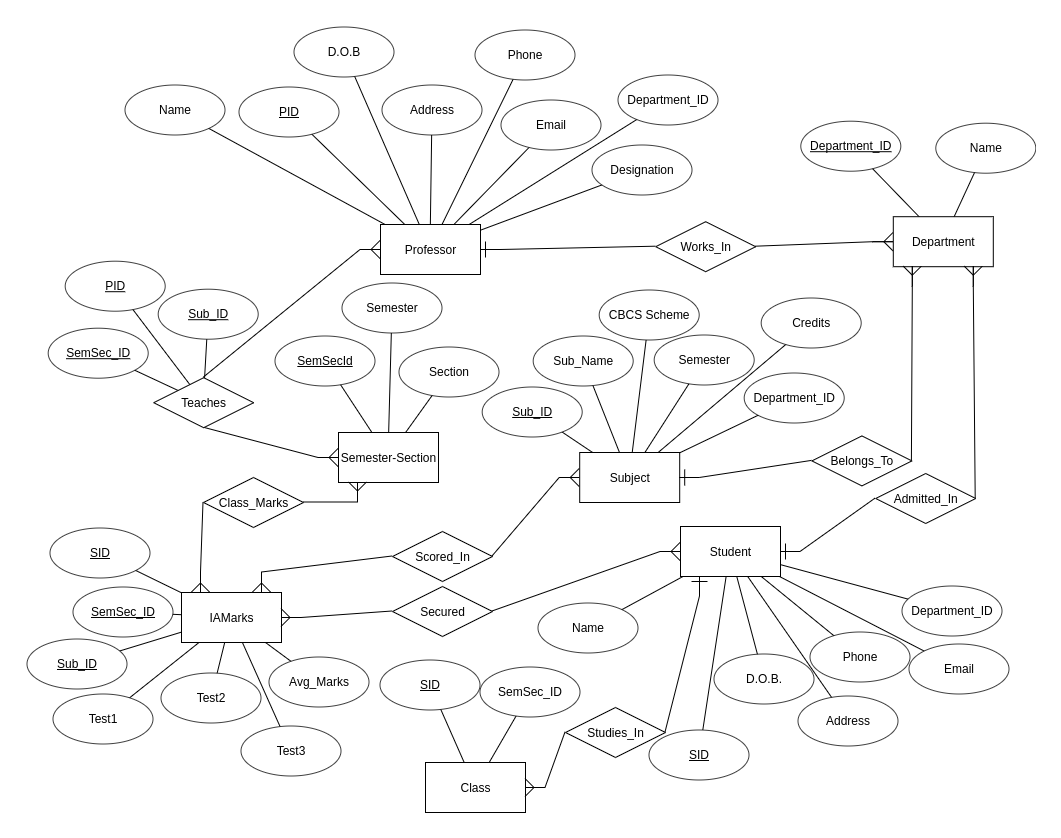
\includegraphics[scale=0.47]{./erd.png}
\label{fig:ER diagram}
\end{figure}

\thispagestyle{fancy}

\section{Relational Schema}
\begin{figure}[H]
\centering
\caption{Relational Schema}
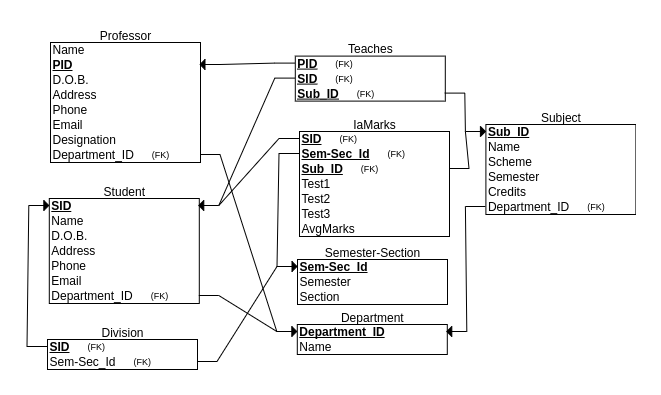
\includegraphics[scale=.7]{./schema.png}
\\[0.2in]
\label{fig:Relational Schema}
\end{figure}

\thispagestyle{fancy}

\chapter{DESCRIPTION OF TOOLS AND TECHNOLOGIES}

\section{JavaFX}
JavaFX is a software platform for creating and delivering desktop applications, as well as rich Internet applications (RIAs) that can run across a wide variety of devices. JavaFX is intended to replace Swing as the standard GUI library for Java SE, but both will be included for the foreseeable future. JavaFX has support for desktop computers and web browsers on Microsoft Windows, Linux, and macOS.\\

JavaFX applications could run on any desktop that could run Java SE or on any mobile phone that could run Java ME.

\thispagestyle{fancy}

\section{Java}
Java is a general-purpose computer programming language that is concurrent,
class-based, object-oriented, and specifically designed to have as few implementation dependencies as possible. It is intended to let application developers "write once, run anywhere" (WORA), meaning that compiled Java code can run on all platforms that support Java without the need for recompilation. Java applications are typically compiled to bytecode that can run on any Java virtual machine (JVM) regardless of computer architecture.\\

As of 2016, Java is one of the most popular programming languages in use, particularly for client-server web applications, with a reported 9 million developers.\\

Java was originally developed by James Gosling at Sun Microsystems (which has since been acquired by Oracle Corporation) and released in 1995 as a core component of Sun Microsystems' Java platform. The language derives much of its syntax from C and C++, but it has fewer low-level facilities
than either of them.\\

One design goal of Java is portability, which means that programs written for the Java platform must run similarly on any combination of hardware and operating system with adequate runtime support. This is achieved by compiling the Java language code to an intermediate representation called Java bytecode, instead of directly to architecture-specific
machine code. Java bytecode instructions are analogous to machine code, but they are intended to be executed by a virtual machine (VM) written specifically for the host hardware. End users commonly use a Java Runtime Environment (JRE) installed on their own machine for standalone Java applications, or in a web browser for Java applets.

\thispagestyle{fancy}

\section{MySQL}
MySQL is a Relational Database Management System (RDBMS). MySQL server can
manage many databases at the same time. In fact, many people might have different databases managed by a single MySQL server. Each database consists of a structure to hold the data and the data itself. A data-base can exist without data, only a structure, be totally empty, twiddling its thumbs and waiting for data to be stored in it.\\

Data in a database is stored in one or more tables. You must create the data-base and the tables before you can add any data to the database. First you create the empty database. Then you add empty tables to the database. Database tables are organized like other tables that you’re used in rows and columns. Each row represents an entity in the database, such as a customer, a book, or a project. Each column contains an item of information about the entity, such as a customer name, a book name, or a project start date. The place where a particular row and column intersect, the individual cell of the table, is called a field. Tables in databases can be related. Often a row in one table is related to several rows in another table.\\

For instance, you might have a database containing data about books you own. You would have a book table and an author table. One row in the author table might contain information about the author of several books in the book table. When tables are related, you include a column in one table to hold data that matches data in the column of another table. MySQL, the most popular Open Source SQL database management system, is developed, distributed, and supported by MySQL AB. MySQL AB is a commercial company, founded by the MySQL developers. It is a second generation Open Source company that unites Open Source values and methodology with a successful business model.
\pagestyle{fancy}
\begin{itemize}
	\item MySQL is a database management system. A database is a structured collection of data. It may be anything from a simple shopping list to a picture gallery or the vast	amounts of information in a corporate network. To add, access, and process data stored in a computer database, you need a database management system such as	MySQL Server. Since computers are very good at handling large amounts of data,
	database management systems play a central role in computing, as standalone utilities, or as parts of other applications.
	
	\item MySQL is a relational database management system. A relational database stores data in separate tables rather than putting all the data in one big storeroom. This adds speed and flexibility. The SQL part of “MySQL” stands for “Structured Query Language.” SQL is the most common standardized language used to access databases and is defined by the ANSI/ISO SQL Standard. The SQL standard has been evolving since 1986 and several versions exist. “SQL-92” refers tothe standard released in	1992, “SQL:1999” refers to the standard released in 1999, and “SQL:2003” refers to the current version of the standard. We use the phrase “the SQLstandard” to mean the current version of the SQL Standard at any time.
	
	\item MySQL software is Open Source. Open Source means that it is possible for anyone to use and modify the software. Anybody can download the MySQL software from the Internet and use it without paying anything. If you wish, you may study the source code and change it to suit your needs. The MySQL software uses the GPL (GNU General Public License), to define what you may and may not do with the software in
	different situations. The MySQL Database Server is very fast, reliable, and easy to use.
	
	\item MySQL Server works in client/server or embedded systems. The MySQL Database Software is a client/server system that consists of a multi-threaded SQL server that supports different back ends, several different clientprograms and libraries, administrative tools, and a wide range of application programming interfaces (APIs).
	\end{itemize}

\thispagestyle{fancy}

\chapter{JAVA DATABASE CONNECTIVITY}
\thispagestyle{fancy}
Java Database Connectivity (JDBC) is an application programming interface (API) for the programming language Java, which defines how a client may access a database. It is Java based data access technology and used for Java database connectivity. It is part of the Java Standard Edition platform, from Oracle Corporation. It provides methods to query and
update data in a database, and is oriented towards relational databases. A JDBC-to-ODBC bridge enables connections to any ODBC-accessible data source in the Java virtual machine (JVM) host environment.

\section{Functionality}
JDBC allows multiple implementations to exist and be used by the same application. The API provides a mechanism for dynamically loading the correct Java packages and registering them with the JDBC Driver Manager. The Driver Manager is used as a connection factory for creating JDBC connections.\\
JDBC connections support creating and executing statements. These may be update statements such as SQL's CREATE, INSERT, UPDATE and DELETE, or they may be query statements such as SELECT. Additionally, stored procedures may be invoked through a JDBC connection. JDBC represents statements using one of the following classes:
\begin{itemize}
	\item Statement – the statement is sent to the database server each and every time.
	\item PreparedStatement – the statement is cached and then the execution path is pre-determined on the database server allowing it to be executed multiple times in an efficient manner.
	\item CallableStatement – used for executing stored procedures on the database.
\end{itemize}
Update statements such as INSERT, UPDATE and DELETE return an update count that indicates how many rows were affected in the database. These statements do not return any other information.\\
Query statements return a JDBC row result set. The row result set is used to walk over the result set. Individual columns in a row are retrieved either by name or by column number. There may be any number of rows in the result set. The row result set has meta data that describes the names of the columns and their types. There is an extension to the basic JDBC
API in the javax.sql. JDBC connections are often managed via a connection pool rather than obtained directly from the driver.

\section{JDBC DRIVERS}
JDBC drivers are client-side adapters (installed on the client machine, not on the server) that convert requests from Java programs to a protocol that the DBMS can understand. Types Commercial and free drivers provide connectivity to most relational-database servers. These drivers fall into one of the following types:
\begin{itemize}
	\item \textbf{Type 1} that calls native code of the locally available ODBC driver.
	\item \textbf{Type 2} that calls database vendor native library on a client side. This code then talks to database over the network.
	\item \textbf{Type 3} the pure-java driver that talks with the server-side middleware that then talks to the database.
	\item \textbf{Type 4} the pure-java driver that uses database native protocol.
\end{itemize}
Note also a type called an internal JDBC driver - a driver embedded with JRE in Java-enabled SQL databases which is used for Java stored procedures.

\thispagestyle{fancy}
\section{Steps to connect to the database in Java}
There are 5 steps to connect any java application with the database in java using JDBC.\\

They are as follows:
\begin{itemize}
\item Register the driver class
\item Creating connection
\item Creating statement
\item Executing queries
\item Closing connection
\end{itemize}

\subsection{Register the driver class}
The forName() method of Class class is used to register the driver class. This method is used to dynamically load the driver class.\\

Syntax of forName() method :\\
public static void forName(String className ) throws ClassNotFoundException\\

\subsection{Create the connection object}
The getConnection() method of DriverManager class is used to establish connection with the database.\\

\noindent Syntax of getConnection() method:\\
• public static Connection getConnection(String url)throws SQLException\\
• public static Connection getConnection(String url,String name,String password) throws SQLException
\subsection{Create the Statement object}
The createStatement() method of Connection interface is used to create statement. The object of statement is responsible to execute queries with the database.\\

\noindent Syntax of createStatement() method:\\
public Statement createStatement() throws SQLException
\subsection{Execute the query}
The executeQuery() method of Statement interface is used to execute queries to the database. This method returns the object of ResultSet that can be used to get all the records of a table.\\

\noindent Syntax of executeQuery() method:\\
public ResultSet executeQuery(String sql) throws SQLException
\subsection{Close the connection object}
By closing connection object statement and ResultSet will be closed automatically. The close() method of Connection interface is used to close the connection.\\

\noindent Syntax of close() method:\\
public void close() throws SQLException

\thispagestyle{fancy}

\chapter{IMPLEMENTATION}
\setstretch{1}
\section{Code For Major Functionalities}
\subsection{Database Operation}
\thispagestyle{fancy}

\begin{lstlisting}[caption=DatabaseContract.java]
public class DatabaseContract {
  public static final String ROW_ID = "_ROWID";
  public static final String ROW_ID_DATA_TYPE = "BIGINT(8) UNSIGNED NOT NULL UNIQUE AUTO_INCREMENT";
  public static final String PROCEDURE_IA_MARKS_CALCULATE_AVERAGE = "IA_MARKS_CALCULATE_AVERAGE";
  public static final String SQL_IA_MARKS_CALCULATE_AVERAGE = "CREATE PROCEDURE " + PROCEDURE_IA_MARKS_CALCULATE_AVERAGE + "()\n" +
      "BEGIN\n" +
      " DECLARE a, b, c, average INT;\n" +
      " DECLARE done INT DEFAULT FALSE;\n" +
      " DECLARE id BIGINT(8);\n" +
      " DECLARE cur CURSOR FOR\n" +
      " SELECT " + DatabaseContract.ROW_ID + ", " + DatabaseContract.IaMarks.TEST1 + ", " + DatabaseContract.IaMarks.TEST2 + ", " + DatabaseContract.IaMarks.TEST3 + " FROM " + DatabaseContract.IaMarks.TABLE_NAME + ";\n" +
      " DECLARE CONTINUE HANDLER FOR NOT FOUND SET done = TRUE;  \n" +
      " OPEN cur;\n" +
      "   m_loop : LOOP\n" +
      "     SET done = FALSE;\n" +
      "     FETCH cur INTO id, a, b, c;\n" +
      "     IF(done) THEN\n" +
      "       LEAVE m_loop;\n" +
      "     END IF;\n" +
      "     SET average = (a+b+c)/3;\n" +
      "     UPDATE college.IA_MARKS SET AVG_MARKS = average WHERE " + DatabaseContract.ROW_ID + " = id;\n" +
      "     SET done = done+1;\n" +
      "   END LOOP;\n" +
      " CLOSE cur;\n" +
      "END\n";

  public class Professor {
    public static final String TABLE_NAME = "PROFESSOR";
    public static final String NAME = "NAME";
    public static final String PROFESSOR_ID = "PROFESSOR_ID";
    public static final String DATE_OF_BIRTH = "DATE_OF_BIRTH";
    public static final String ADDRESS = "ADDRESS";
    public static final String PHONE = "PHONE";
    public static final String EMAIL = "EMAIL";
    public static final String DEPARTMENT_ID = "DEPARTMENT_ID";
    public static final String DESIGNATION = "DESIGNATION";
  }

  public class Department {
    public static final String TABLE_NAME = "DEPARTMENT";
    public static final String NAME = "NAME";
    public static final String DEPARTMENT_ID = "DEPARTMENT_ID";
  }

  public class Student {
    public static final String TABLE_NAME = "STUDENT";
    public static final String NAME = "NAME";
    public static final String STUDENT_ID = "STUDENT_ID";
    public static final String DATE_OF_BIRTH = "DATE_OF_BIRTH";
    public static final String ADDRESS = "ADDRESS";
    public static final String PHONE = "PHONE";
    public static final String EMAIL = "EMAIL";
    public static final String DEPARTMENT_ID = "DEPARTMENT_ID";
  }

  public class Subject {
    public static final String TABLE_NAME = "SUBJECT";
    public static final String NAME = "NAME";
    public static final String SUBJECT_ID = "SUBJECT_ID";
    public static final String SCHEME = "SCHEME";
    public static final String SEMESTER = "SEMESTER";
    public static final String SEMESTER_IDX = "SEMESTER_IDX";
    public static final String CREDITS = "CREDITS";
    public static final String CREDITS_IDX = "CREDITS_IDX";
    public static final String DEPARTMENT_ID = "DEPARTMENT_ID";
 }

  public class SemesterSection {
    public static final String TABLE_NAME = "SEMESTER_SECTION";
    public static final String SEM_SEC_ID = "SEM_SEC_ID";
    public static final String SEMESTER = "SEMESTER";
    public static final String SEMESTER_IDX = "SEMESTER_IDX";
    public static final String SECTION = "SECTION";
  }

  public class Division {
    public static final String TABLE_NAME = "DIVISION";
    public static final String STUDENT_ID = "STUDENT_ID";
    public static final String SEM_SEC_ID = "SEM_SEC_ID";
  }

  public class Teaches {
    public static final String TABLE_NAME = "TEACHES";
    public static final String PROFESSOR_ID = "PROFESSOR_ID";
    public static final String SEM_SEC_ID = "SEM_SEC_ID";
    public static final String SUBJECT_ID = "SUBJECT_ID";
  }

  public class IaMarks {
    public static final String TABLE_NAME = "IA_MARKS";
    public static final String STUDENT_ID = "STUDENT_ID";
    public static final String SEM_SEC_ID = "SEM_SEC_ID";
    public static final String SUBJECT_ID = "SUBJECT_ID";
    public static final String TEST1 = "TEST1";
    public static final String TEST1_IDX = "TEST1_IDX";
    public static final String TEST2 = "TEST2";
    public static final String TEST2_IDX = "TEST2_IDX";
    public static final String TEST3 = "TEST3";
    public static final String TEST3_IDX = "TEST3_IDX";
    public static final String AVG_MARKS = "AVG_MARKS";
    public static final String AVG_MARKS_IDX = "AVG_MARKS_IDX";
  }
}
\end{lstlisting}

\begin{lstlisting}[caption=DatabaseHelper.java]
package com.nagpal.shivam.dbms.data;

import com.nagpal.shivam.dbms.Log;
import com.nagpal.shivam.dbms.data.DatabaseContract.*;
import com.nagpal.shivam.dbms.model.*;

import java.sql.*;
import java.util.ArrayList;
import java.util.List;

public class DatabaseHelper {


  public static final String SEARCH_MODE_NATURAL_LANGUAGE = "Natural Language Mode";
  public static final String SEARCH_MODE_BOOLEAN = "Boolean Mode";
  private static final String CLASS_NAME = DatabaseHelper.class.getSimpleName();

  public static List<DepartmentData> fetchDepartmentDetails() {
    String sql = "SELECT * FROM " +
        Department.TABLE_NAME;
    Connection connection = Database.getConnection();
    List<DepartmentData> list = new ArrayList<>();
    try {
      Statement statement = connection.createStatement();
      ResultSet set = statement.executeQuery(sql);
      int rowIdIndex = set.findColumn(DatabaseContract.ROW_ID);
      int nameIndex = set.findColumn(Department.NAME);
      int departmentIdIndex = set.findColumn(Department.DEPARTMENT_ID);

      while (set.next()) {
        list.add(new DepartmentData(set.getLong(rowIdIndex), set.getString(nameIndex), set.getString(departmentIdIndex)));
      }
    } catch (SQLException e) {
      Log.e(CLASS_NAME, e.getMessage());
    }
    return list;
  }

  public static List<DepartmentData> fetchParticularDepartment(String departmentId, boolean include) {
    String operator = include ? " = " : " != ";
    String sql = "SELECT * FROM " +
        Department.TABLE_NAME +
        " WHERE " +
        Department.DEPARTMENT_ID + operator + "'" + departmentId + "'";
    Connection connection = Database.getConnection();
    List<DepartmentData> list = new ArrayList<>();
    try {
      Statement statement = connection.createStatement();
      ResultSet set = statement.executeQuery(sql);
      int rowIdIndex = set.findColumn(DatabaseContract.ROW_ID);
      int nameIndex = set.findColumn(Department.NAME);
      int departmentIdIndex = set.findColumn(Department.DEPARTMENT_ID);

      while (set.next()) {
        list.add(new DepartmentData(set.getLong(rowIdIndex), set.getString(nameIndex), set.getString(departmentIdIndex)));
      }
    } catch (SQLException e) {
      Log.e(CLASS_NAME, e.getMessage());
    }
    return list;
  }

  public static List<DepartmentData> searchDepartmentDetails(String searchString, String mode) {
    String sql = "SELECT * FROM " +
        Department.TABLE_NAME +
        " WHERE MATCH(" + Department.NAME + "," + Department.DEPARTMENT_ID + ") " +
        "AGAINST(? IN " + mode.toUpperCase() + ")";
    Connection connection = Database.getConnection();
    List<DepartmentData> list = new ArrayList<>();
    try {
      PreparedStatement preparedStatement = connection.prepareStatement(sql);
      preparedStatement.setString(1, searchString);
      ResultSet set = preparedStatement.executeQuery();
      int rowIdIndex = set.findColumn(DatabaseContract.ROW_ID);
      int nameIndex = set.findColumn(Department.NAME);
      int departmentIdIndex = set.findColumn(Department.DEPARTMENT_ID);

      while (set.next()) {
        list.add(new DepartmentData(set.getLong(rowIdIndex), set.getString(nameIndex), set.getString(departmentIdIndex)));
      }
    } catch (SQLException e) {
      Log.e(CLASS_NAME, e.getMessage());
    }
    return list;
  }

  public static int updateDepartment(DepartmentData departmentData) {
    String sql = "UPDATE " +
        Department.TABLE_NAME +
        " SET " +
        Department.NAME + "=?, " +
        Department.DEPARTMENT_ID + "=? " +
        "WHERE " + DatabaseContract.ROW_ID + " =" + departmentData.rowId;
    Connection connection = Database.getConnection();
    try {
      PreparedStatement statement = connection.prepareStatement(sql);
      statement.setString(1, departmentData.name);
      statement.setString(2, departmentData.departmentId);
      statement.executeUpdate();
    } catch (SQLException e) {
      Log.e(CLASS_NAME, e.getMessage());
      return e.getErrorCode();
    }
    return SqlErrorCodes.SQLITE_OK;
  }

  public static int deleteRow(String tableName, long rowId) {
    String sql = "DELETE FROM " +
        tableName +
        " WHERE " + DatabaseContract.ROW_ID + " =" + rowId;
    Connection connection = Database.getConnection();
    try {
      Statement statement = connection.createStatement();
      statement.execute(sql);
    } catch (SQLException e) {
      Log.e(CLASS_NAME, e.getMessage());
      return e.getErrorCode();
    }
    return SqlErrorCodes.SQLITE_OK;
  }

  public static int executeIaMarksCalculateAverage() {
    String sql = "{CALL " + DatabaseContract.PROCEDURE_IA_MARKS_CALCULATE_AVERAGE + "()}";
    Connection connection = Database.getConnection();
    try {
      CallableStatement statement = connection.prepareCall(sql);
      statement.execute();
    } catch (SQLException e) {
      Log.e(CLASS_NAME, e.getMessage());
      return e.getErrorCode();
    }
    return SqlErrorCodes.SQLITE_OK;
  }
}

\end{lstlisting}


\pagebreak
\subsection{Model Class}
\thispagestyle{fancy}
\begin{lstlisting}[caption=DepartmentData.java]
package com.nagpal.shivam.dbms.model;

import com.nagpal.shivam.dbms.data.PreviewIgnoredAttribute;

public class DepartmentData {
  @PreviewIgnoredAttribute
  public long rowId;
  public String name;
  public String departmentId;

  public DepartmentData() {
  }

  public DepartmentData(String name, String departmentId) {
    this.name = name;
    this.departmentId = departmentId;
  }

  public DepartmentData(long rowId, String name, String departmentId) {
    this.rowId = rowId;
    this.name = name;
    this.departmentId = departmentId;
  }
  
}
\end{lstlisting}


\pagebreak
\subsection{UI Scenes}
\thispagestyle{fancy}
\begin{lstlisting}[caption=PreviewDatabase.java]
package com.nagpal.shivam.dbms.ui;

import com.nagpal.shivam.dbms.navigation.Intent;
import com.nagpal.shivam.dbms.navigation.NavUtil;
import javafx.scene.Scene;
import javafx.scene.control.Button;
import javafx.scene.image.Image;
import javafx.scene.image.ImageView;
import javafx.scene.layout.*;

import java.util.ArrayList;
import java.util.LinkedHashMap;
import java.util.Map;

import static com.nagpal.shivam.dbms.Main.sStage;

public class PreviewDatabase extends UiScene {
  @Override
  public void setScene() {
    Pane pane = getLayout();
    pane.getStyleClass().add("parentPane");
    Scene scene = new Scene(pane);
    scene.getStylesheets().add("css/PreviewDatabaseScene.css");
    sStage.setTitle("Database Preview");
    sStage.setScene(scene);
    pane.requestFocus();
  }

  @Override
  protected Pane getLayout() {
    Image logo = new Image("images/college-pic.png");
    ImageView logoImageView = new ImageView(logo);
    logoImageView.setFitWidth(400);
    logoImageView.setFitHeight(300);
    FlowPane logoImageViewFlowPane = new FlowPane(logoImageView);
    logoImageViewFlowPane.getStyleClass().add("logoImageViewFlowPane");

    LinkedHashMap<String, Class> linkedHashMap = new LinkedHashMap<>();
    linkedHashMap.put("Professor", PreviewProfessor.class);
    linkedHashMap.put("Student", PreviewStudent.class);
    linkedHashMap.put("Department", PreviewDepartment.class);
    linkedHashMap.put("Subject", PreviewSubject.class);
    linkedHashMap.put("Division", PreviewDivision.class);
    linkedHashMap.put("Teaches", PreviewTeaches.class);
    linkedHashMap.put("Semester-Section", PreviewSemesterSection.class);
    linkedHashMap.put("IaMarks", PreviewIaMarks.class);
    TilePane tilePane = new TilePane();

    ArrayList<Button> buttons = new ArrayList<>();
    for (Map.Entry<String, Class> entry : linkedHashMap.entrySet()) {
      Button button = new Button(entry.getKey());
      button.setOnAction(event -> NavUtil.startScene(new Intent(PreviewDatabase.this, entry.getValue())));
      buttons.add(button);
    }

    tilePane.setPrefColumns(3);
    tilePane.setHgap(20);
    tilePane.setVgap(20);
    tilePane.getChildren().addAll(buttons);

    FlowPane tileFlowPane = new FlowPane(tilePane);
    tileFlowPane.getStyleClass().add("tileFlowPane");

    VBox vBox = new VBox(logoImageViewFlowPane, tileFlowPane);
    vBox.setSpacing(30);

    BorderPane borderPane = new BorderPane();
    borderPane.setCenter(vBox);
    return borderPane;
  }
}

\end{lstlisting}

\pagebreak
\subsection{CSS}
\thispagestyle{fancy}
\begin{lstlisting}[caption=PreviewDatabase.css]
.parentPane {
    -fx-min-width: 800;
    -fx-min-height: 600;
}

.logoImageViewFlowPane {
    -fx-alignment: center;
}

.tileFlowPane {
    -fx-alignment: center;
}

.button {
    -fx-pref-width: 200;
    -fx-background-radius: 100;
    -fx-padding: 20;
    -fx-alignment: center;
}

\end{lstlisting}


\chapter{Snapshots}
\setstretch{1.5}
\section{Login Scene}
\begin{figure}[H]
\caption{Login Scene}
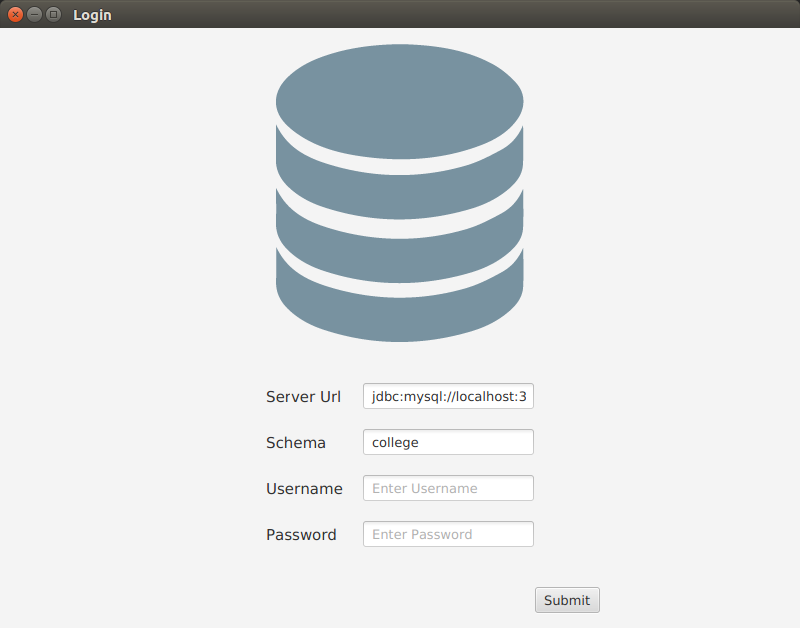
\includegraphics[scale=.6]{./login.png}
\label{fig:Login Scene}
\end{figure}

\thispagestyle{fancy}


\section{Database Preview Scene}
\begin{figure}[H]
\caption{Database Preview Scene}
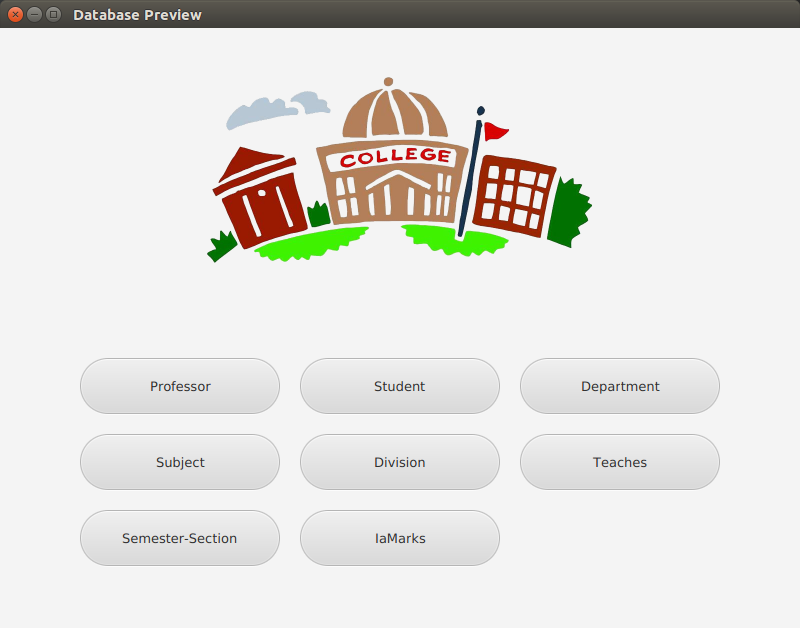
\includegraphics[scale=0.6]{./database_preview.png}
\label{fig:Database Preview Scene}
\end{figure}

\section{Relation Preview Scene}
\begin{figure}[H]
\caption{Relation Preview Scene}
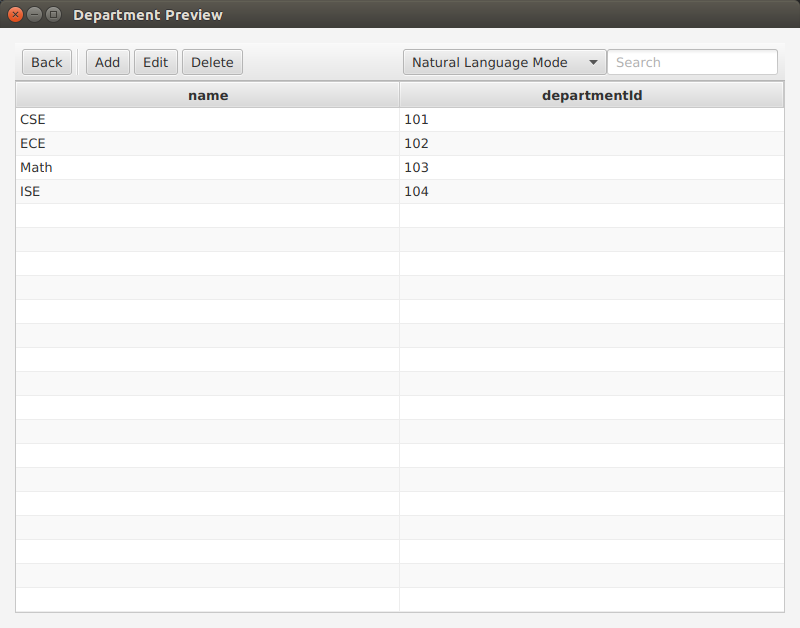
\includegraphics[scale=0.6]{./relation_preview.png}
\label{fig:Relation Preview Scene}
\end{figure}

\section{Add New Entry Scene}
\begin{figure}[H]
\caption{Add New Entry Scene}
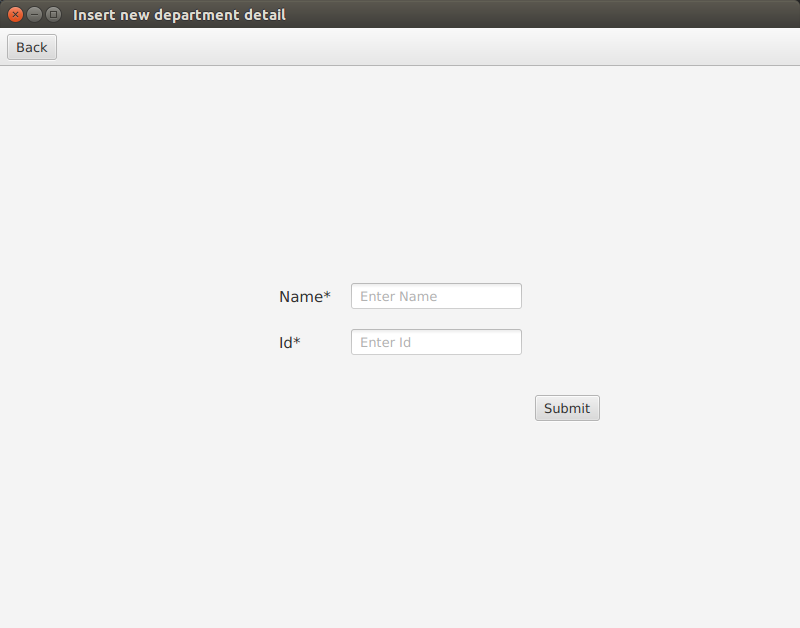
\includegraphics[scale=0.6]{./add_new_entry.png}
\label{fig:Add New Entry Scene}
\end{figure}

\section{Edit Entry Scene}
\begin{figure}[H]
\caption{Edit Entry Scene}
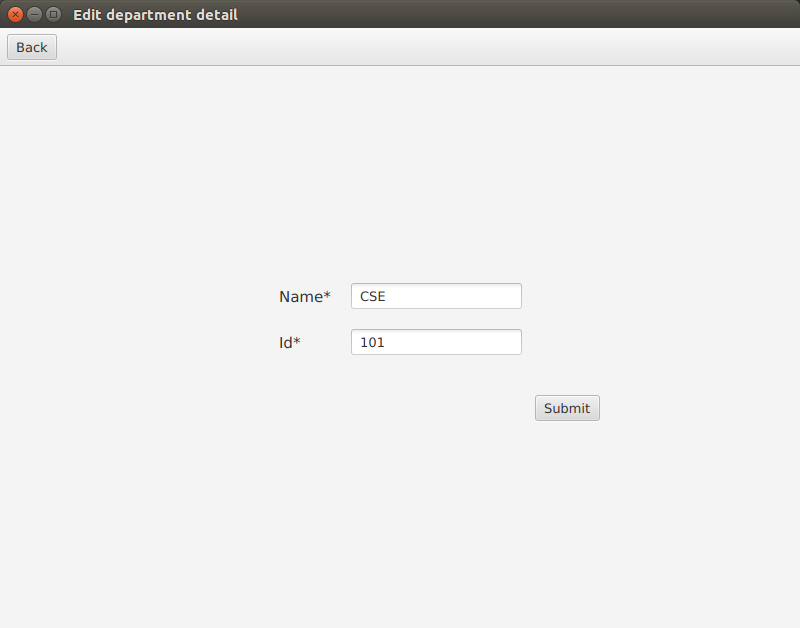
\includegraphics[scale=0.6]{./edit_entry.png}
\label{fig:Edit Entry Scene}
\end{figure}

\section{Search Modes}
\begin{figure}[H]
\caption{Search Modes}
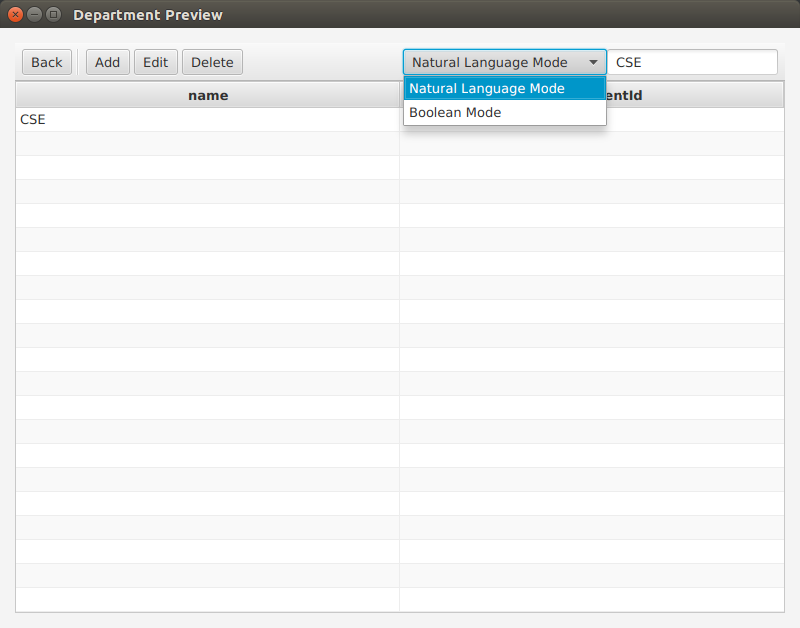
\includegraphics[scale=0.6]{./search_mode.png}
\label{fig:Search Modes}
\end{figure}
\chapter{Conclusion and Future Enhancements}
This project is a rather rudimentary implementation of a larger system.
We have been successful in automating the core objective of this project.

Enhancements that we would like to explore in the future:
\begin{itemize}
\item Integrating all college related entities to make it universal solution
\item Implement graph plotting for better visualization of data
\item Auto Completion and Scheduling of tasks for better work flow
\end{itemize}
\pagebreak

\cleardoublepage
%\pagebreak
\phantomsection
\begin{flushleft}
	
\begin{thebibliography}{99}
	
\bibitem{}Fundamentals of database systems by (Elmasri Navathe, 2000)\\

\bibitem{} Java: \url{https://docs.oracle.com/en/java/}\\

\bibitem{} MySQL: \url{https://www.mysql.com/}\\

\bibitem{}System Analysis and Design: \url{https://www.tutorialspoint.com/system_analysis_and_design/}\\
\end{thebibliography}

\end{flushleft}


\end{document}
